\documentclass[12pt,a4paper]{article}

%Encoding
\usepackage[utf8]{inputenc}

%Matemática
\usepackage{amsmath,amsfonts,amssymb}

%Formato de página
\usepackage[margin=1.5cm,footskip=20pt]{geometry}

%Misc
\usepackage{url}

%Código fuente
 \usepackage{listings}
\usepackage[usenames,dvipsnames]{xcolor}

%Figuras
\usepackage{graphicx}
\usepackage{float}
\usepackage{subcaption}

%Apendices
\usepackage{appendix}
\renewcommand{\appendixname}{Anexos}
\renewcommand{\appendixtocname}{Anexos}
\renewcommand{\appendixpagename}{Anexos}



\title{Práctica numérica Física Teórica 3: \\ Modelado de Ising 2D por Monte Carlo Metropolis}
\author{E. A. Galpern, S. Schiavinato}
\date{\today}

\begin{document}

\maketitle



\section{Introducción}

\subsection{Modelo físico}
El modelo de Ising en dos dimensiones (2D) corresponde un modelo de ferromagnetismo en materiales a partir de consideraciones cuánticas simples. El modelo es usado principalmente por su simplicidad y porque demuestra propiedades interesantes al variar la temperatura del material. 

El modelo consiste en tener $N$ spines, que pueden ser partículas compuestas o simples, colocadas en una matriz cuadrada. Los spines posibles son dos, que vamos a llamar $+$ y $-$ (y en el algoritmo identificamos así), donde abstraímos la unidad del momento dipolar magnético; este proceso es muy común en simulaciones numéricas. 

El modelo propone que el sentido del spín queda determinado mediante la interacción de la partícula con sus vecinas y por fluctuaciones térmicas. De esa forma,  interesa obtener los observables macroscópicos de la energía, magnetización y sus variaciones, por sitio (para normalizar a un valor independiente del tamaño de la red) 

El hamiltoneano del modelo corresponde a 

\begin{equation}
    H\,=\,-J\sum_{<i,j>}\sigma_i\sigma_j
\end{equation}

donde la suma sobre $<i,j>$ considera solamente a los vecinos, sin contabilizar más de una vez. Además, el modelo propone condiciones de contorno periódicas. El signo de $J$, que es una constante de normalización, determina si la iteracción es ferromagnética o antiferromagnética, es decir, si la menor energía corresponde a alinear o desalinear los spines

Veamos un poco el espectro de ese hamiltoneano, ya que vamos a usar algunas conclusiones. Supongamos que tenemos todos los spines apuntando hacia arriba, esto es $\sigma_i = +1$; en ese caso, la energía total es $-2 N J$. Para ello se piensa que cada posición tiene cuatro vecinos. Si se procede así, se contó dos veces, por lo finalmente que hay que dividir por dos. De esta forma la energía del estado fundamental será $H_0=-2JN$. El primer estado excitado es que un sólo espín apunte hacia abajo, con energía $H_1=-2JN + 8J$ y así sucesivamente. 

 Si dos spines vecinos apuntan en la misma dirección su energía mutua es $-J$, lo que reduce la energía del sistema. Por tanto, la interacción que hemos puesto tiende a hacer que los spines apunten en la misma dirección, ya que disminuye la energía total. Esto lo que hace es favorecer la aparición de la magnetización total. Podríamos pensar que hemos resuelto ya el problema: la magnetización tiene que valer siempre $m=1$ para minimizar la energía y ya está.

Sin embargo, tenemos que recordar que el problema está planteado en el ensamble canónico, esto es, a temperatura constante (el volumen no juega un papel crucial, ya que los spines de la retícula no desaparecen o aparecen). En estas condiciones, la termodinámica nos indica el equilibrio no vendrá dada por un mínimo de energía, sino por un mínimo de la energía libre \[F=U-T\,S\].

El estado fundamental minimiza la energía $U$, pero es un estado ordenado, por lo que la entropía es máxima. Si la temperatura es baja, el producto $T\,S$ lo es, y a la energía libre contribuye sobre todo la energía: el sistema se magnetizará espontáneamente a baja temperatura. Sin embargo cuando sube la temperatura la entropía comienza a tomar importancia, por lo que minimizar la energía libre pasa por maximizar la entropía. Justamente el estado más desordenado posible (de mayor entropía), es aquel con la mitad de espines hacia arriba y la mitad hacia abajo, es decir con magnetización por sitio nula, $m = 0$. 

Con este mismo argumento podemos decir que la energía tendrá un mínimo a temperatura alta y un máximo a temperatura baja, para lo cual debe haber un cambio en la concavidad al considerar la energía como función de la temperatura. Esto implica una discontinuidad en el calor específico, además de que será nulo a temperatura baja y alta.

La solución exacta, o una solución numérica, nos dirá exactamente a qué temperatura empieza a gestarse la transición entre un estado y otro, llamado comunmente transición de fase. Esta es la temperatura crítica, o simplemente $T_c$.

La solución exacta de Onsager considera que el límite termodinámico $N \to \infty$ en sus cálculos, obteniendo la siguiente temperatura crítica.

\begin{equation}
   T_c=\frac{2J}{k_B\log(\sqrt{2}+1)} = 2.269 J
   \label{eq:t_onsager}
\end{equation}

Sabiendo la temperatura crítica buscaremos observar las simulaciones numéricas buscando un cambio en la magnetización.

Para completar mostramos los observables en función de la temperatura, deducidos de la solución de Onsager, que se pueden ver en la figura \ref{fig:onsager}

\begin{figure}[H]
\begin{subfigure}[c]{0.45\textwidth}
\centering
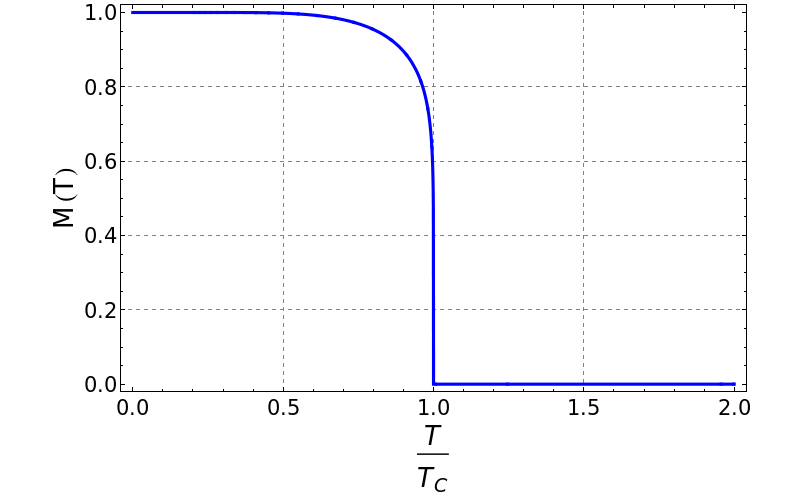
\includegraphics[width=\textwidth]{teoricos/m_onsager.png}
\caption{Magnetizacion por sitio}
\label{fig:m_onsager}
\end{subfigure}
\begin{subfigure}[c]{0.45\textwidth}
\centering
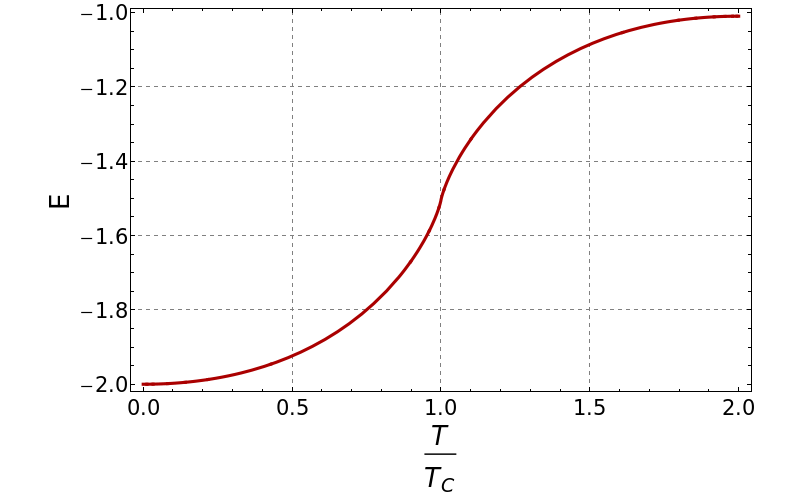
\includegraphics[width=\textwidth]{teoricos/e_onsager.png}
\caption{Energía por sitio}
\label{fig:e_onsager}
\end{subfigure}
\\
\centering
\begin{subfigure}[c]{0.45\textwidth}
\centering
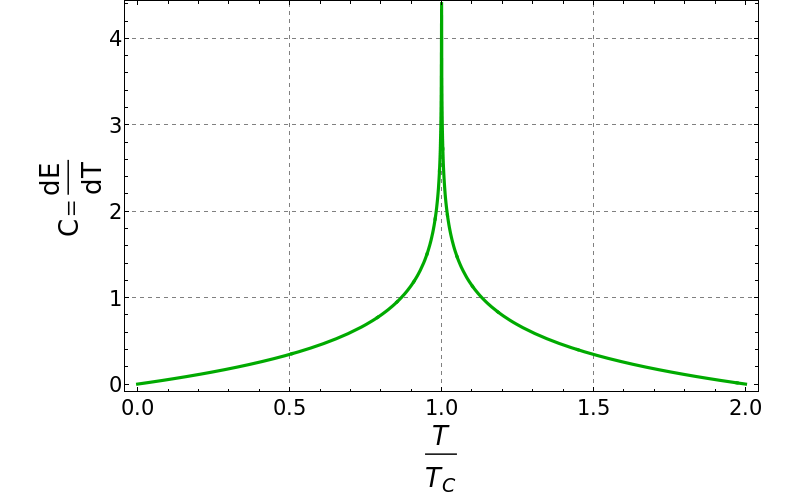
\includegraphics[width=\textwidth]{teoricos/c_onsager.png}
\caption{Capacidad calórica}
\label{fig:c_onsager}
\end{subfigure}
\caption{Observables en función de la temperatura adimensional deducidos de la solución de Onsager}
\label{fig:onsager}
\end{figure}


\subsection{Exponentes críticos}
Usando la aproximación de campo medio podemos encontrar que la magnetización sigue una relación de \emph{scaling}
\begin{equation}
 m \propto (T_C - T)^{\beta}
 \label{eq:exp_critico}
\end{equation}
con un exponente crítico $\beta = 0.5$

\subsection{Método de Monte Carlo Metropolis}

El método de Monte Carlo consiste en una forma de calcular valores medios, a partir de la simulación de la dinámica del sistema. La idea consiste en encontrar todas los posibles estados del sistema, considerando el macroestado en equilibrio, por medio del siguiente algoritmo
\begin{enumerate}
\item Inicializar la red
\item Elegir un spin al azar o de forma ordenada.
\item Observar el cambio de energía al cambiar el spin de sentido.
\item Aceptar el cambio con una probabilidad de transición $P(x \to x')$.
\item Medir los observables.
\item Repetir las veces necesarias desde el paso 2.
\end{enumerate}
El método propone que al ir avanzando con el algoritmo se va a poder observar todos los estados posibles (o una cantidad apreciable de estados), concepto que se conoce comúnmente como \emph{ergodicidad}. Para que la elección de estados sea coherente debemos elegir una probabilidad de transición coherente, pero por suerte naturalmente encontramos que
\begin{equation}
  P(x \to x') = 
  \begin{cases}
    1 & \text{si } E_{x'} - E_x \leq 0 \\
    e^{-\beta (E_{x'} - E_x)} & \text{si } E_{x'} - E_x > 0
  \end{cases}.
\end{equation}
Este transición asegura que si la energía del estado nuevo es menor, entonces el estado nuevo es aceptado si o si, y si no se considera la probabilidad canónica $e^{-\beta E}$. Ahora corresponde determinar cómo calculamos el valor de $E_{x'} - E_{x}$, al hacer el cambio de un sólo spin
\begin{equation}
    E_{x'} - E_{x} = \Delta E = -J \sum_{<n,r>} s_n s_r - (-J) \sum_{<i,r>} s_i s_r =  2 J s_i \sum_{<j>} s_j 
\end{equation}

es decir se pasa a sumar sólamente sobre la energía asociada a los vecinos del spin que se está cambiando. Esto permite simplificar la implementación del algoritmo



\section{Resultados}

\subsection{Termalizado}
En este apartado vamos a observar cuantos pasos hay que descartar hasta llegar a un estado de equilibrio. En nuestra simulación, al inicializar la red dispusimos todos los spines ordenados, por lo que a temperatura debajo de la temperatura crítica el sistema termaliza casi desde el paso inicial. De sea forma, no nos pareció interesante mostrar la termalización para esas temperaturas. En la figura \ref{fig:term_256} podemos ver la magnetización paso a paso desde el estado inicial para una red de 256 por 256 spines

\begin{figure}[H]
\begin{subfigure}[c]{0.45\textwidth}
\centering
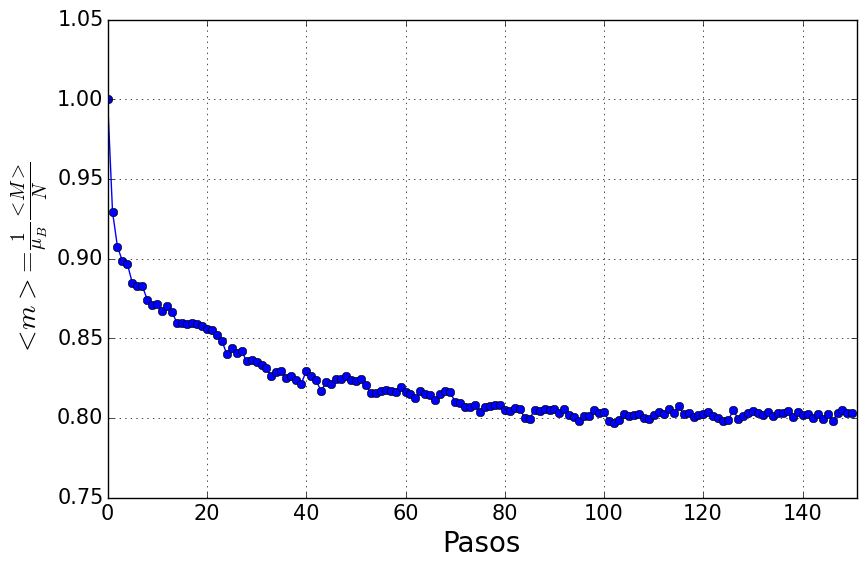
\includegraphics[width=\textwidth]{termalizado/term_L_256_tc.png}
\caption{$T \approx T_C$}
\label{fig:term_256_tc}
\end{subfigure}
\begin{subfigure}[c]{0.45\textwidth}
\centering
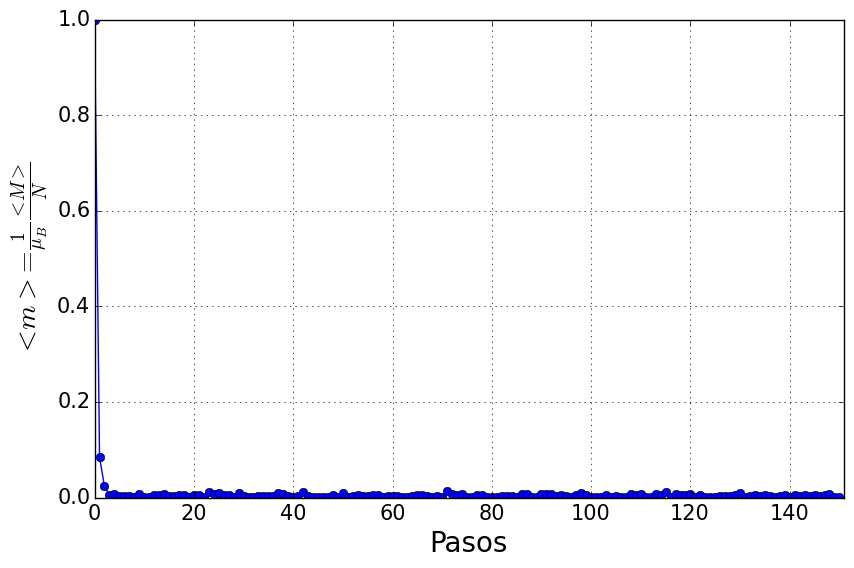
\includegraphics[width=\textwidth]{termalizado/term_L_256_5tc.png}
\caption{$T \approx 5 T_C$}
\label{fig:term_256_5tc}
\end{subfigure}
\caption{Magnetización medida paso a paso de la simulación Monte Carlo para una red de 256 x 256}
\label{fig:term_256}
\end{figure}

Se nota claramente que la temperatura crítica aumenta considerablemente la cantidad de pasos antes de termalizar, ya que el estado inicial no tiene ninguna correlación con el estado de equilibrio. Sin embargo, con 100 pasos aproximadamente podemos asumir que se llega a termalizar la red.
%eze: esto ya no describe las figuras. 

Comparemos con una red más pequeña, de 64 por 64, que podemos ver en la figura \ref{fig:term_64}.

\begin{figure}[H]
\begin{subfigure}[c]{0.45\textwidth}
\centering
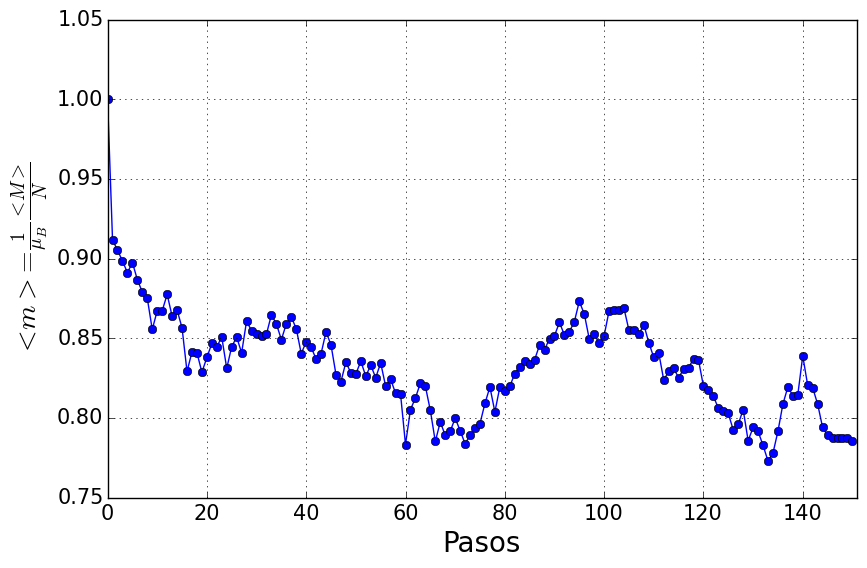
\includegraphics[width=\textwidth]{termalizado/term_L_64_tc.png}
\caption{$T \approx T_C$}
\label{fig:term_64_tc}
\end{subfigure}
\begin{subfigure}[c]{0.45\textwidth}
\centering
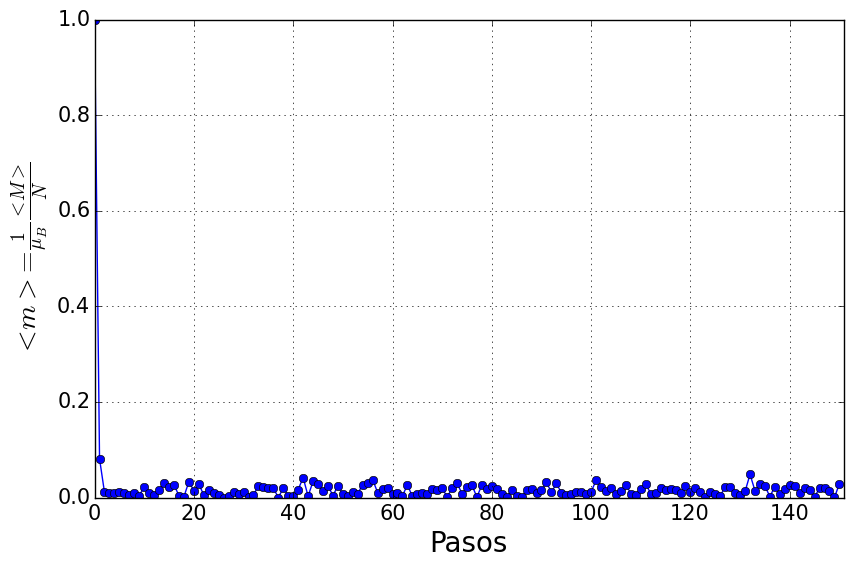
\includegraphics[width=\textwidth]{termalizado/term_L_64_5tc.png}
\caption{$T \approx 5 T_C$}
\label{fig:term_64_5tc}
\end{subfigure}
\caption{Magnetización medida paso a paso de la simulación Monte Carlo para una red de 64$\times$64}
\label{fig:term_64}
\end{figure}

Acá queda claro que en una red más pequeña es necesario más pasos previos antes de termalizar y que existe aún más variación de la magnetización en la temperatura crítica.
%DISCUTIR
%Eso es debido a que al aumentar la cantidad de spines en la red en cada paso de Monte Carlo, usando el código anterior, se comparan más configuraciones posibles, avanzando más la termalización

\section{Observables}
Ahora presentamos para dos tamaños de redes los observables en función de la temperatura. Después de termalizar se mide los observables varias veces para obtener un promedio "temporal". Además tomamos mediciones cada cierta cantidad de pasos, para impedir que influya la correlación entre pasos. Tomamos 200 mediciones cada 100 pasos.
%No hicimos el análisis de cambiar la cantidad de pasos entre mediciones.

En la figura  \ref{fig:obs_L_8}   y la figura \ref{fig:obs_L_128} presentamos la magnetización, la energía y el calor específico para una red de 8$\times$8 y de  128$\times$128 respectivamente.

\begin{figure}[H]
\begin{subfigure}[c]{0.45\textwidth}
\centering
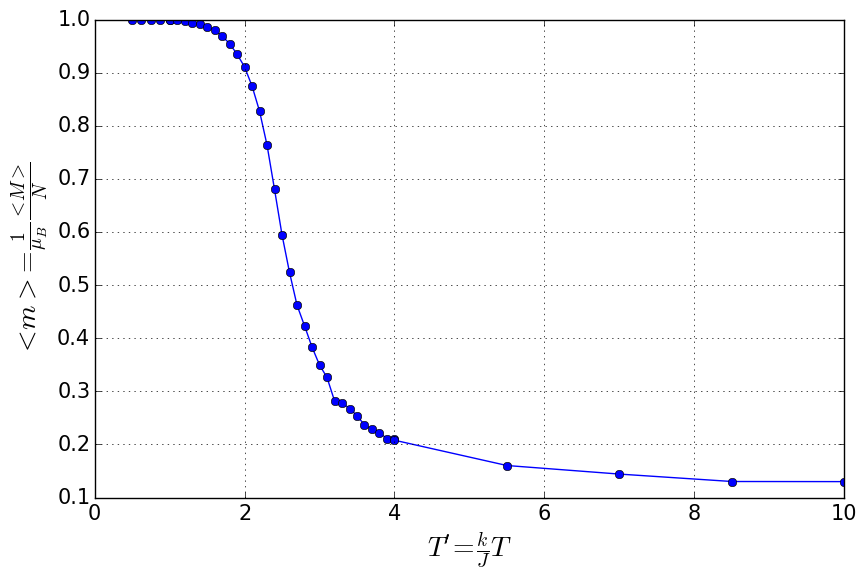
\includegraphics[width=\textwidth]{observables/mag_L_8.png}
\caption{Magnetizacion por sitio}
\label{fig:mag_L_8}
\end{subfigure}
\begin{subfigure}[c]{0.45\textwidth}
\centering
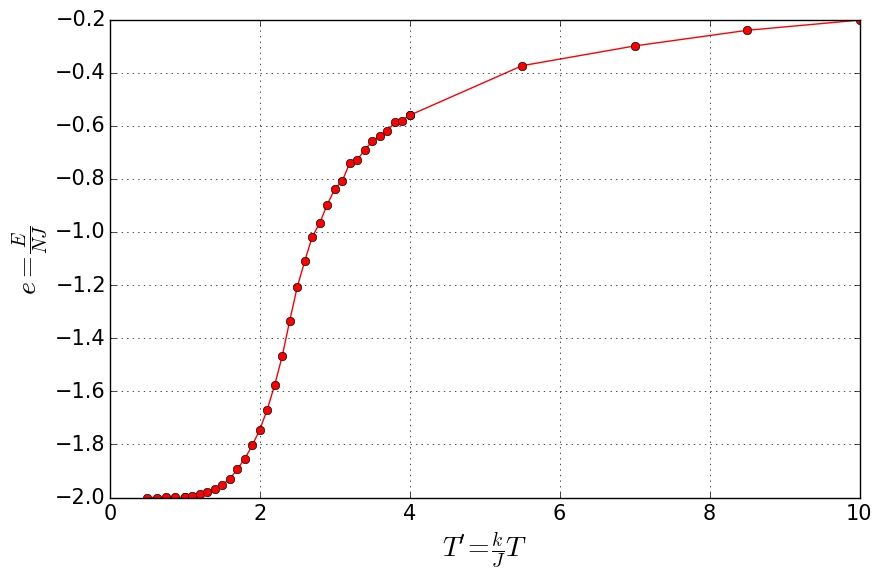
\includegraphics[width=\textwidth]{observables/e_L_8.png}
\caption{Energía por sitio}
\label{fig:e_L_8}
\end{subfigure}
\\
\centering
\begin{subfigure}[c]{0.45\textwidth}
\centering
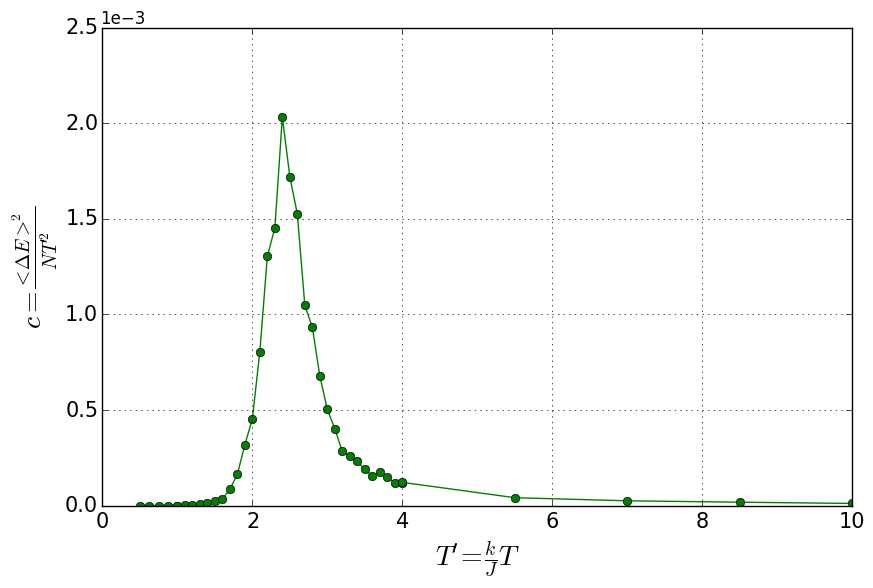
\includegraphics[width=\textwidth]{observables/c_L_8.png}
\caption{Capacidad calorífica}
\label{fig:c_L_8}
\end{subfigure}
\caption{Observables en función de la temperatura adimensional para una red de 8 x 8}
\label{fig:obs_L_8}
\end{figure}


\begin{figure}[H]
\begin{subfigure}[c]{0.45\textwidth}
\centering
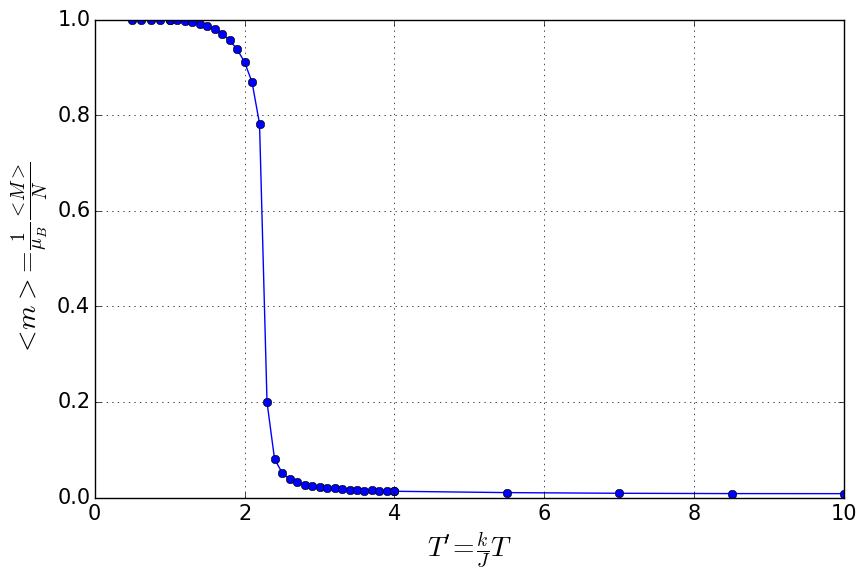
\includegraphics[width=\textwidth]{observables/mag_L_128.png}
\caption{Magnetizacion por sitio}
\label{fig:mag_L_128}
\end{subfigure}
\begin{subfigure}[c]{0.45\textwidth}
\centering
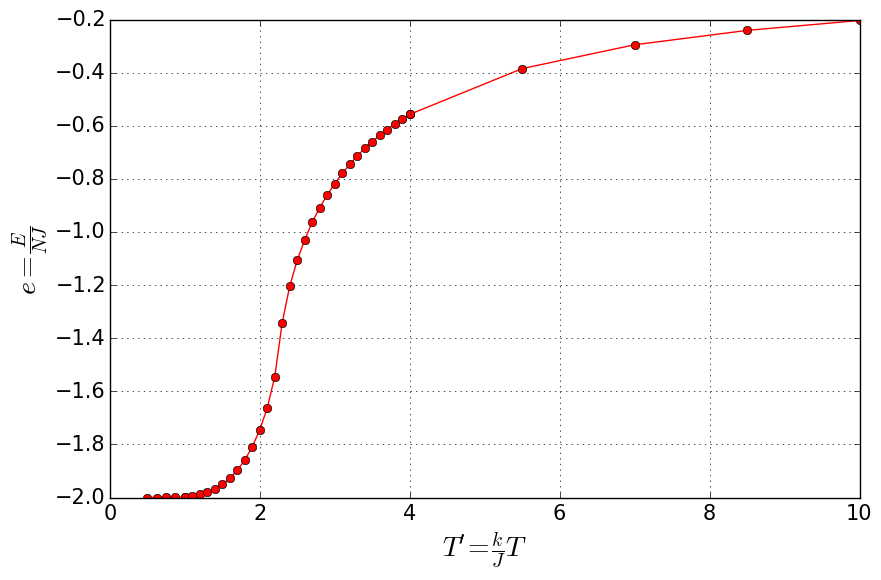
\includegraphics[width=\textwidth]{observables/e_L_128.png}
\caption{Energía por sitio}
\label{fig:e_L_128}
\end{subfigure}
\\
\centering
\begin{subfigure}[c]{0.4\textwidth}
\centering
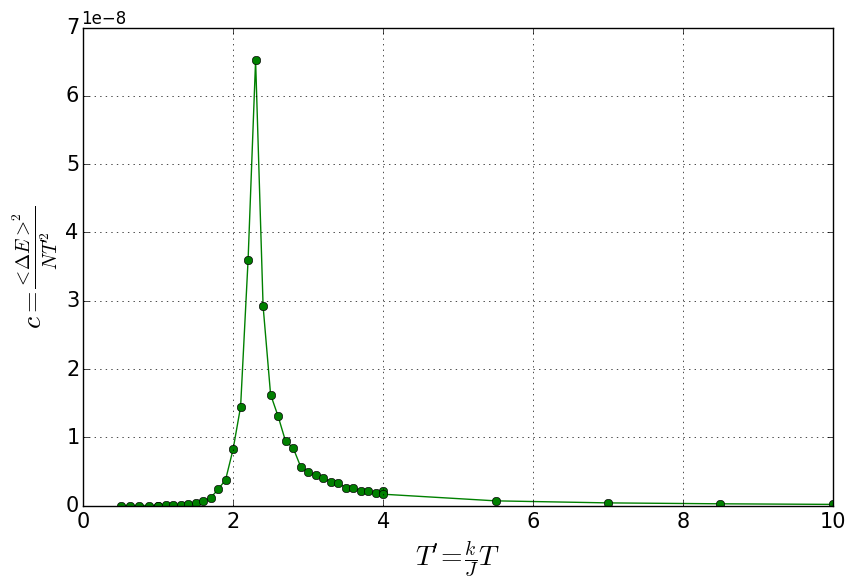
\includegraphics[width=\textwidth]{observables/c_L_128.png}
\caption{Capacidad calorífica}
\label{fig:c_L_128}
\end{subfigure}
\caption{Observables en función de la temperatura adimensional para una red de 128 x 128}
\label{fig:obs_L_128}
\end{figure}

En estas figuras podemos ver los comportamientos esperados de la magnetización y la energía para ambos casos, sin ser totalmente nula la magnetización para la red de 8$\times$8, ni ser totalmente discontinua en ambos casos. Esto demuestra que no hay una transición de fase real para estos tamaños de red, pero al serguir seguir aumentado se acerca al comportamiento.
Para comparar los calores específico  presentamos en la figura \ref{fig:c_L} el calor específico en función de la temperatura para diferentes tamaños de red. Para poder observar mejor los gráficos se normalizaron los calores específicos.

\begin{figure}[H]
\centering
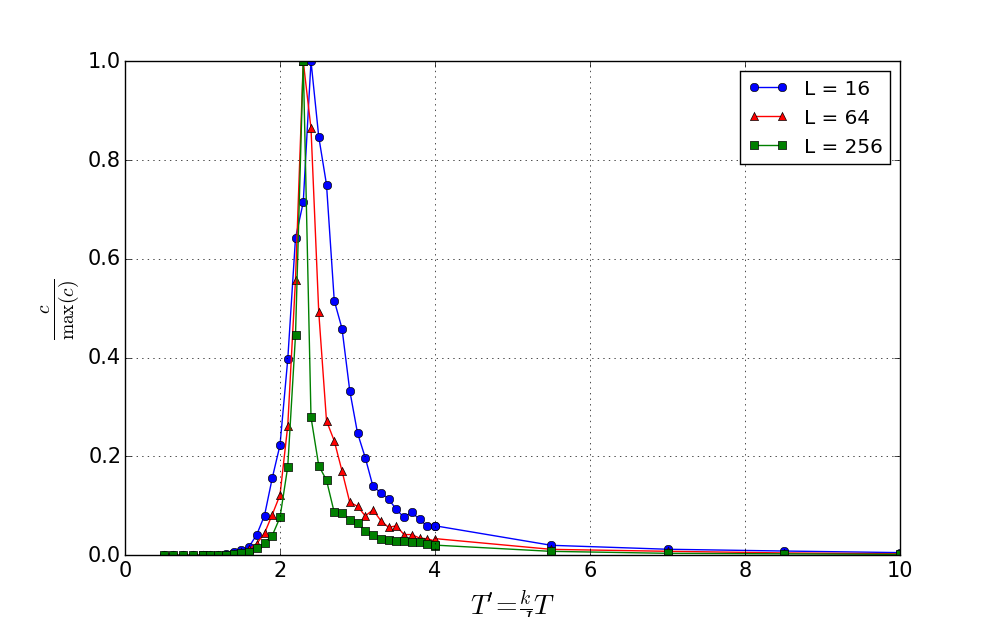
\includegraphics[width = 0.6\textwidth]{observables/c_L_8_16_256}
\caption{Calor específico en función de la temperatura para diversos tamaños de red}
\label{fig:c_L}
\end{figure}

Nuevamente observamos el mismo comportamiento: al aumentar la cantidad de spines en la red se acerca más al comportamiento propio de la transición de fase. Esto es totalmente consistente con la solución de Onsager, ya que en ella se tomó el paso al límite termodinámico $N = L \times L \to \infty$ que por una realidad numérica no podemos hacer en la simulación.

\section{Exponentes críticos}
Para poder observar si se corresponde los exponentes críticos ahora graficamos la magnetización en función de la temperatura, con un ajuste de la función
\[ f(T, T_c, A, \beta) = A (T_c - T)^\beta.\]
En la figura \ref{fig:m_ajuste} mostramos los datos ajustados

\begin{figure}[H]
\centering
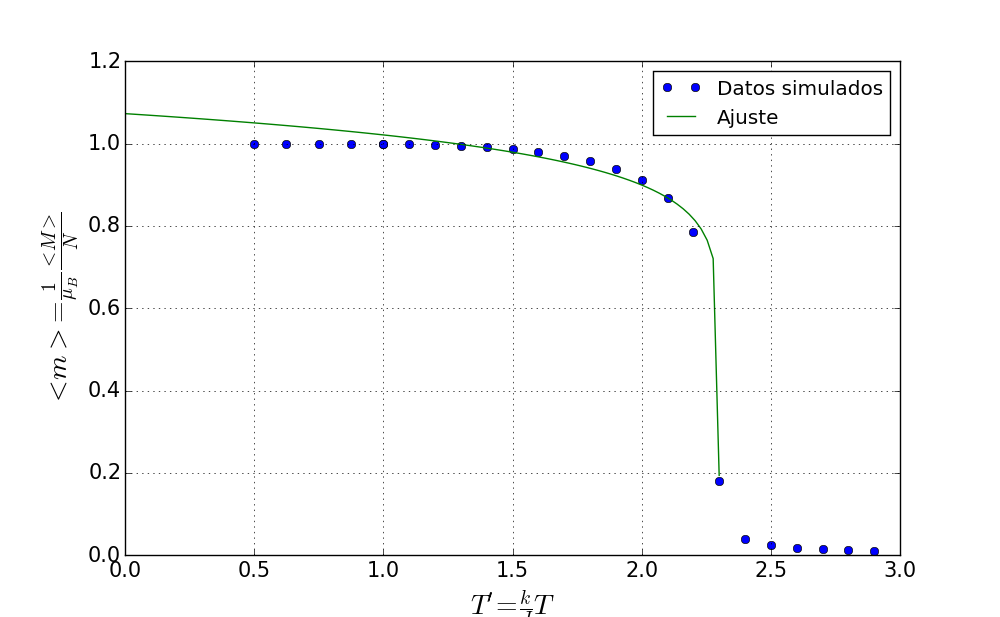
\includegraphics[width = 0.6\textwidth]{observables/m_ajuste.png}
\caption{Magnetización con un ajuste una ley de potencia efectuado}
\label{fig:m_ajuste}
\end{figure}

con los parámetros observados en la tabla \ref{tbl:m_ajuste}
\begin{table}[H]
\centering
\begin{tabular}{c|c}
 Parámetro & Ajuste \\\hline
 $T_c$ & 2,229 \\
 $\beta$ & 0,086 \\
 A & 0,998 \\
\end{tabular}
\caption{Ajustes de la figura \ref{fig:m_ajuste}}
\label{tbl:m_ajuste}
\end{table}

Podemos ver que la temperatura crítica es parecida a la encontrada analíticamente en la solución de Onsager (vista en la ecuación \ref{eq:t_onsager}), pero el exponente crítico es un orden de magnitud menor al esperado (0,5 como vimos en la ecuación \ref{eq:exp_critico}). Esto puede ser a la elección de las temperaturas a medir y los datos ajustados, ya que la relación de scaling funciona cerca de la temperatura crítica.

\section{Conclusiones}
Pudimos implementar un algoritmo de Monte Carlo Metrópolis para realizar simulaciones numéricas con un Modelo de Ising en dos dimensiones de un material ferromagnético para redes de distinto tamaño.

A partir de este método, encontramos que al llegar a la temperatura crítica aumenta considerablemente la cantidad de pasos antes de termalizar y que en una red más pequeña son necesarios más pasos previos.
Por otra parte, medimos la magnetización, el calor específico y la energía cada 100 pasos, repetidas veces para tomar promedios "temporales". Encontramos los comportamientos que se acercan a lo esperado de la magnetización y la energía, aunque la magnetización no llegara a anularse para la red de 8$\times$8, ni ser totalmente discontinua en todos los casos. Concluimos que no hay una transición de fase real para estos redes de hasta 128$\times$128, pero al serguir seguir aumentado el tamaño nos aproximamos al comportamiento esperado.
En el caso del Calor específico, al aumentar la cantidad de spines en la red se acerca más al comportamiento propio de la transición de fase. Esto es totalmente consistente con la solución de Onsager, ya que en ella se tomó el paso al límite termodinámico $N = L \times L \to \infty$ que por una realidad numérica no podemos hacer en la simulación.
Por último, analizamos los exponentes críticos ajustando la magnetización como una ley de potencias de la temperatura, encontrando que la temperatura crítica es parecida a la encontrada analíticamente en la solución de Onsager (vista en la ecuación \ref{eq:t_onsager}), pero el exponente crítico es un orden de magnitud menor al esperado. Concluimos que esto podría deberse a la elección de las temperaturas a medir y los datos ajustados, ya que la relación de scaling funciona cerca de la temperatura crítica.


\clearpage % o \cleardoublepage
\addappheadtotoc

\appendixpage

\appendix

\section{Código fuente}

El programa para simular este proceso fue escrito en Julia, un lenguaje de programación de alto nivel compilado con orientación al cálculo científico, versión 0.3. La sintaxis es muy parecida al Matlab y Python, tomando lo mejor de ambos entornos.
No presentamos el código utilizado para graficar los datos, así como el código para guardarlos. Todos esos datos están disponibles en el repositorio \url{http://github.com/sadeus/ft3_df_uba}.

%Setea los caracteres extraños para listing
\lstset{literate=
  {á}{{\'a}}1 {é}{{\'e}}1 {í}{{\'i}}1 {ó}{{\'o}}1 {ú}{{\'u}}1
  {Á}{{\'A}}1 {É}{{\'E}}1 {Í}{{\'I}}1 {Ó}{{\'O}}1 {Ú}{{\'U}}1
  {à}{{\`a}}1 {è}{{\`e}}1 {ì}{{\`i}}1 {ò}{{\`o}}1 {ù}{{\`u}}1
  {À}{{\`A}}1 {È}{{\'E}}1 {Ì}{{\`I}}1 {Ò}{{\`O}}1 {Ù}{{\`U}}1
  {ä}{{\"a}}1 {ë}{{\"e}}1 {ï}{{\"i}}1 {ö}{{\"o}}1 {ü}{{\"u}}1
  {Ä}{{\"A}}1 {Ë}{{\"E}}1 {Ï}{{\"I}}1 {Ö}{{\"O}}1 {Ü}{{\"U}}1
  {â}{{\^a}}1 {ê}{{\^e}}1 {î}{{\^i}}1 {ô}{{\^o}}1 {û}{{\^u}}1
  {Â}{{\^A}}1 {Ê}{{\^E}}1 {Î}{{\^I}}1 {Ô}{{\^O}}1 {Û}{{\^U}}1
  {œ}{{\oe}}1 {Œ}{{\OE}}1 {æ}{{\ae}}1 {Æ}{{\AE}}1 {ß}{{\ss}}1
  {ç}{{\c c}}1 {Ç}{{\c C}}1 {ø}{{\o}}1 {å}{{\r a}}1 {Å}{{\r A}}1
  {€}{{\EUR}}1 {£}{{\pounds}}1 {ñ}{{\~n}}1 {Ñ}{{\~N}}1
}

%% Coloreado para Julia
\lstdefinelanguage{Julia}%
  {morekeywords={abstract,break,case,catch,const,continue,do,else,elseif,%
      end,export,false,for,function,immutable,import,importall,if,in,%
      macro,module,otherwise,quote,return,switch,true,try,type,typealias,%
      using,while},%
   sensitive=true,%
   alsoother={$},%
   morecomment=[l]\#,%
   morecomment=[n]{\#=}{=\#},%
   morestring=[s]{"}{"},%
   morestring=[m]{'}{'},%
}[keywords,comments,strings]%

\lstset{%
    language         = Julia,
    basicstyle       = \ttfamily,
    keywordstyle     = \bfseries\color{blue},
    stringstyle      = \color{magenta},
    commentstyle     = \color{ForestGreen},
    showstringspaces = false,
}
{\footnotesize
\begin{lstlisting}[inputencoding=utf8,extendedchars=true]
import PyPlot #ploteo de datos
using LaTeXStrings #Permite usar LaTeX en los strings

#Funciones auxiliares. 
#Nota: Los arrays son pasados por referencia.
#Entonces, no es necesario retornarlos con return

#Función que calcula el cambio de energía al cambiar el spin i
# deltaE =  2 * i * (abajo + arriba + izquierda + derecha)
function deltaE(latt, i)
    L = size(latt)[1]
    N = L * L
    #Condiciones de contorno
    i_down = i % L != 0 ? i + 1 : i - L + 1
    i_up = (i - 1) % L != 0 ? i - 1 : i + L - 1
    i_izq = (i - L) > 0 ? i - L : i - L + N
    i_der = (i + L) <= N ? i + L : i + L - N
    result = latt[i_up] 
    result += latt[i_down]
    result += latt[i_izq] 
    result += latt[i_der]
    result *= 2 * latt[i] 
    return result
end

#Función que implementa la transición entre configuraciones.
#Se ejecuta en cada paso de Monte Carlo y recorre N spines al azar o ordenado
function transicion(latt, T, isRandom = false)
    srand(time_ns())
    L = size(latt)[1] #Tamaño de la red
    N = L * L 
    beta = 1.0 / T
    p = [exp(-beta * 4), exp(-beta * 8)]
    for s = 1:N
            #Permite elegir un spin al azar o ordenadamente
            if isRandom
                i = rand(1:L)
            else
                i = s
            end
            dE = deltaE(latt, i)
            if dE != 0 #No hacer nada si dE = 0
                if dE < 0 || p[dE == 4 ? 1 : 2] > rand()
                    latt[i] *= -1                
                end
            end
        end
end

#Función que inicializa la red de L x L. 
#De forma aleatoria o ordenada
function initLatt(L, isRandom = true)
    
     if isRandom
        #Devuelve un número aleatorio de -1:2:1 que es -1,1
        return rand(-1:2:1, L, L)
        #También podemos usar sign(rand(Int32, L, L))
    else
        #Devuelve red ordenada con unos.
        return ones(L, L)
    end
end

#Funcion utilizada para medir observables
function sampleo(latt)
    
    L = size(latt)[1]
    N = L * L
    m = 0.0
    e = 0.0
    m = sum(latt) #Con sumar es suficiente
    for i = 1:N
        #Multiplica con los vecinos posteriores.
        i_der = (i + L) <= N ? i + L : i + L - N
        i_down = i % L != 0 ? i + 1 : i - L + 1
        e += latt[i] * (latt[i_der] + latt[i_down])
    end
    m /= N
    e /= N
    return (abs(m), e) #Tomo sólo la magnitud de la magnetización
end

#Función donde se implementa la iteración Monte Carlo
function isingMetropolis(L, T, fMed = 100, nSamp = 1000, nTerm = 500, 
                        lattRandom = false, randTrans = false) 
    #Cantidad de iteraciones
    nIter = nSamp * fMed  
    N = L*L   
    latt = initLatt(L, lattRandom) #Inicializa la red
    #Observables
    e = zeros(nSamp + 1)
    mag = zeros(nSamp + 1)
    nSamp = 1 #Resteo el nSamp así lo uso como un indice para los observables
    #Termalizado de la red
    for s = 1:nTerm
        #En cada iteración efecutúa una transición posible
        transicion(latt, T, randTrans)
    end
    #Primera medición
    mag[nSamp], e[nSamp] = sampleo(latt)
    nSamp += 1
    for s = 1:nIter
        #En cada iteración efecutúa una transición posible
        transicion(latt,T, randTrans)
        if s % fMed == 0 #Si el paso es múltiplo de fMed => Mide los observables
            mag[nSamp], e[nSamp] = sampleo(latt)
            nSamp += 1
        end
    end
    return (T, mag, e) #Devuelve una tupla con todos los observables
end
\end{lstlisting}
}








\end{document}
